\def\mytitle{CIRCLE ASSIGNMENT}
\def\myauthor{Uday Kumar}
\def\contact{immadisettyudaykumar15@gmail.com}
\def\mymodule{Future Wireless Communication (FWC)}
\documentclass[10pt, a4paper]{article}
\usepackage[a4paper,outer=1.5cm,inner=1.5cm,top=1.75cm,bottom=1.5cm]{geometry}
\twocolumn
\usepackage{graphicx}
\graphicspath{{./images/}}
\usepackage[colorlinks,linkcolor={black},citecolor={blue!80!black},urlcolor={blue!80!black}]{hyperref}
\usepackage[parfill]{parskip}
\usepackage{lmodern}
\usepackage{tikz}
% \usepackage{physics}
%\documentclass[tikz, border=2mm]{standalone}
%\usepackage{karnaugh-map}
%\documentclass{article}
\usepackage{tabularx}
\usepackage{circuitikz}
\usetikzlibrary{calc}
\usepackage{amsmath}
\usepackage{amssymb}
\renewcommand*\familydefault{\sfdefault}
\usepackage{watermark}
\usepackage{lipsum}
\usepackage{xcolor}
\usepackage{listings}
\usepackage{float}
\usepackage{titlesec}
\providecommand{\norm}[1]{\left\lVert#1\right\rVert}
\providecommand{\mtx}[1]{\mathbf{#1}}
\titlespacing{\subsection}{1pt}{\parskip}{3pt}
\titlespacing{\subsubsection}{0pt}{\parskip}{-\parskip}
\titlespacing{\paragraph}{0pt}{\parskip}{\parskip}
\newcommand{\figuremacro}[5]{
    \begin{figure}[#1]
        \centering
        \includegraphics[width=#5\columnwidth]{#2}
        \caption[#3]{\textbf{#3}#4}
        \label{fig:#2}
    \end{figure}
}
\newcommand{\myvec}[1]{\ensuremath{\begin{pmatrix}#1\end{pmatrix}}}
\let\vec\mathbf
\lstset{
frame=single, 
breaklines=true,
columns=fullflexible
}

\title{\mytitle}
\author{\myauthor\hspace{1em}\\\contact\\FWC22086\hspace{6.5em}IITH\hspace{0.5em}\mymodule\hspace{6em}MATRICES}
\date{}
\begin{document}
 \maketitle
 \paragraph*{\large Problem Statement}
$-$ \textbf{ Circles with radii 3,4,5 touch each other externally if P is the point of intersection of tangents to these circles at their point of contact.Find the distance of P from the point of contact.}
 
\begin{figure}[h]
\centering
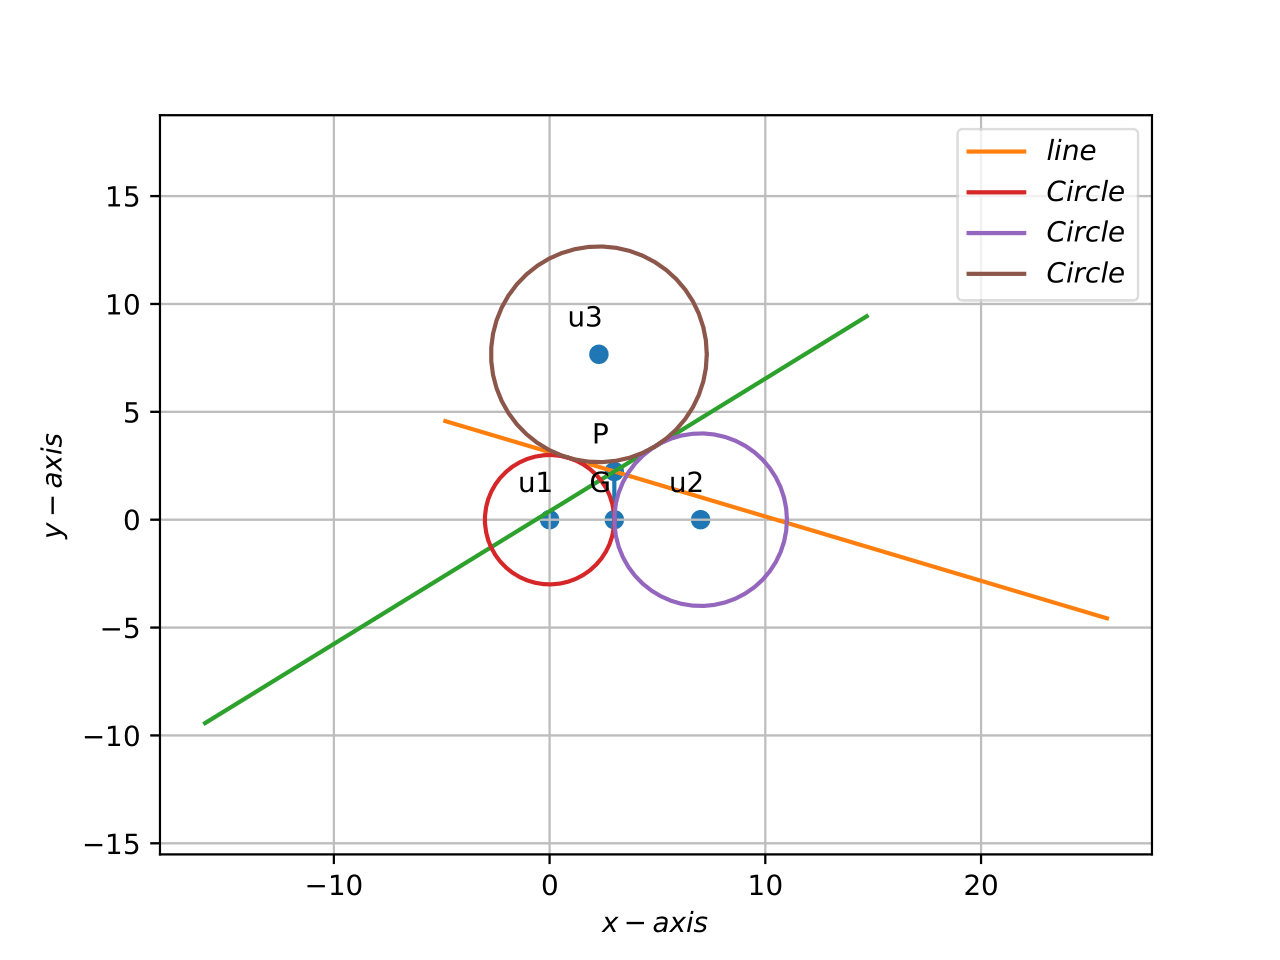
\includegraphics[width=1\columnwidth]{circle1-1.png}
\caption{Perpendcular line}
\end{figure}
 \section*{Construction}
\vspace{2mm}
 The input parameters are as follows
{
\setlength\extrarowheight{4pt}
\begin{center}
 \begin{tabular}{|c|c|c|}
 \hline
 \textbf{Symbol}&\textbf{Value}&\textbf{Description}\\
 \hline
 $r_1$&$
 3$
 &radius  \\
 \hline
 $r_2$&$
 4$
 &radius\\
 \hline
 $r_3$&$
 5$
 &radius\\
 \hline
 $u_1$&$
 \begin{pmatrix}
  0\\
  0\\
 \end{pmatrix}$
 &\\
 \hline
 $u_2$&$
 \begin{pmatrix}
  7\\
  0\\
 \end{pmatrix}$
 &\\
 \hline
 $u_3$&$
 \begin{pmatrix}
  2.28571428751\\
  7.66651878\\
 \end{pmatrix}$
 &$$$e_1$$^T\vec{(a)}$ \\
 \hline
 m&$
 \begin{pmatrix}
  7\\
  0\\
 \end{pmatrix}$
 &$$$e_2$$^T\vec{(b)}$\\
 \hline
 \end{tabular}
 \end{center}
}
\section*{\large solution}

\subsection*{\large step 1}
The general equation of the circle is
\begin{align}
\vec{x}^{\top}\vec{V}\vec{x}+2\vec{u}^{\top}\vec{x}+f=0
\end{align}
where V is the identity matrix
\\Let the equation of the circles with radii 3,4and 5 are 
\begin{align}
\vec{x}^{\top}\vec{x}+2\vec{u_1}^{\top}\vec{x}+f_1=0
\end{align}
\begin{align}
\vec{x}^{\top}\vec{x}+2\vec{u_2}^{\top}\vec{x}+f_2=0
\end{align}
\begin{align}
\vec{x}^{\top}\vec{x}+2\vec{u_3}^{\top}\vec{x}+f_3=0
\end{align}
Common tangent between the circles with $\vec{u_1}$ and $\vec{u_2}$
\begin{align}
2(\vec{u_1}^{\top}-\vec{u_2}^{\top})\vec{x}+f_1-f_2=0
\end{align}
\begin{align}
2(\vec{u_2}^{\top}-\vec{u_3}^{\top})\vec{x}+f_2-f_3=0
\end{align}
\begin{align}
2(\vec{u_3}^{\top}-\vec{u_1}^{\top})\vec{x}+f_3-f_1=0
\end{align}
Solving the above tangent equations we get the  point 
\begin{equation}
\vec{P}=\myvec{3\\2.236}
\end{equation}
\\To find the point of contact ,Foot of the point P to the line formed by the points $\vec{u_1}$ and $\vec{u_2}$
\begin{equation}
\vec{G}=\vec{u_1}+\vec{m}^{\top}\frac{(P-u_1)}{\norm{m}^{2}}\vec{m}
\end{equation}
where
\begin{equation}
\vec{m}=\vec{u_1}-\vec{u_2}
\end{equation}
we get the point 
\begin{equation}
\vec{G}=\myvec{3\\0}
\end{equation}
The distance between the two points G and P is 
\begin{equation}
\vec{D_1} =\norm{\vec{P}-\vec{G}}
\end{equation}
\end{document}
